\def\mytitle{Conics Assignment}
\def\myauthor{A.Gowri Priya}
\def\contact{gowripriyaappayyagari@gmail.com}
\def\mymodule{Future Wireless Communication (FWC)}
\documentclass[10pt, a4paper]{article}
\usepackage[a4paper,outer=1.5cm,inner=1.5cm,top=1.75cm,bottom=1.5cm]{geometry}
\twocolumn
\usepackage{setspace}
\usepackage{graphicx}
\graphicspath{{./images/}}
\usepackage[colorlinks,linkcolor={black},citecolor={blue!80!black},urlcolor={blue!80!black}]{hyperref}
\usepackage[parfill]{parskip}
\usepackage{lmodern}
\usepackage{tikz}
	\usepackage{physics}
%\documentclass[tikz, border=2mm]{standalone}
\usepackage{karnaugh-map}
\usepackage{tabularx}
\usetikzlibrary{calc}
\usepackage{amsmath}
\usepackage{amssymb}
\renewcommand*\familydefault{\sfdefault}
\usepackage{watermark}
\usepackage{lipsum}
\usepackage{xcolor}
\usepackage{listings}
\usepackage{float}
\usepackage{titlesec}
\providecommand{\mtx}[1]{\mathbf{#1}}
\titlespacing{\subsection}{1pt}{\parskip}{3pt}
\titlespacing{\subsubsection}{0pt}{\parskip}{-\parskip}
\titlespacing{\paragraph}{0pt}{\parskip}{\parskip}

\newcommand{\myvec}[1]{\ensuremath{\begin{pmatrix}#1\end{pmatrix}}}
\let\vec\mathbf
\lstset{
frame=single, 
breaklines=true,
columns=fullflexible
}

\title{\mytitle}
\author{\myauthor\hspace{1em}\\\contact\\FWC22012\hspace{6.5em}IITH\hspace{0.5em}\mymodule\hspace{6em}ASSIGN-6}
\date{}
\begin{document}
	\maketitle
\section{Problem}
An ellipse is drawn by taking a diameter of the circle
\begin{math}
(x-1)^2 + y^2=1
\end{math}
 as its semi-minor axis and a diameter of the circle 
 \begin{math}
x^2 + (y-2)^2=4
\end{math} is semi-major axis.If the centre of the ellipse is at the origin and its axes are the coordinate axes, then the equation of the ellipse is?
\section{Construction}
\begin{figure}[h]
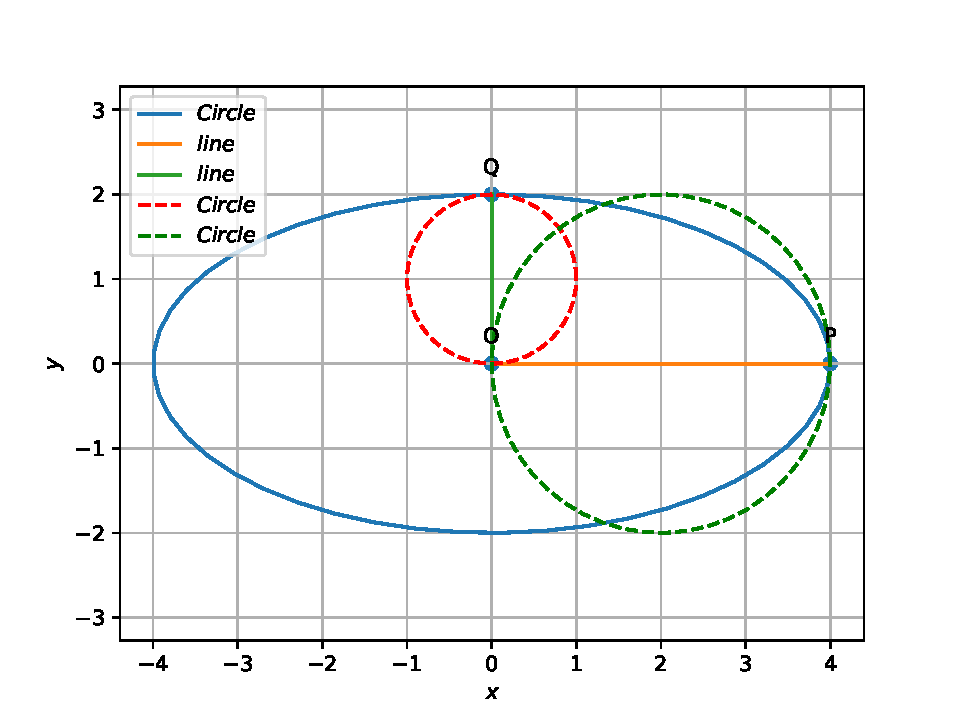
\includegraphics[scale=0.5]{co.pdf} 
\end{figure}
\section{Solution}
Conics equation is 
\begin{equation}
	x^T\vec{V}x + 2\vec{u}^Tx + f = 0
\end{equation}
To find the lengths of semi-major axis and semi-minor axis,\\
From given circle equation \\\\ 
\begin{math}
x^2 + (y-2)^2=4\\\\
x^2+y^2-4y+4=4 \\\\
x^2+y^2-4y=0.....(i)
\end{math}\\\\
By comparing (i) with (1) we will get\\
$\vec{U1}$=$\myvec{0\\-2}$ and f1=0
\begin{equation}
	Radius\;(R) =\sqrt{\vec{u^T}.\vec{u}-f}
\end{equation}
\begin{equation}                                                                                   \sqrt{\myvec{0 &-2}\myvec{0\\-2}} =2                                     
\end{equation}
semi-major axis=2*R=a=4\\\\
From given circle equation \\\\
\begin{math}
(x-1)^2 + (y)^2=1\\\\
x^2+y^2-2x+1=1 \\\\
x^2+y^2-2x=0.....(ii)\\\\
\end{math}\\
By comparing (ii) with (1) we will get\\\\
$\vec{U2}$=$\myvec{-1\\0}$ and f2=0
\begin{equation}
	Radius\;(R) =\sqrt{\vec{u^T}.\vec{u}-f}
\end{equation}
\begin{equation}                                                                                   \sqrt{\myvec{-1 &0}\myvec{-1\\0}} =1                                     
\end{equation}\\
semi-minor axis=2*R=b=2\\\\
For ellipse
given that
\begin{equation}
\vec{U}=\myvec{0\\0}
\end{equation} 
From major axes equation of ellipse\\\\
\begin{equation}
a=\sqrt{(\vec{u^T}.V^-1.\vec{u}-f)/\lambda1}
\end{equation}\\
\begin{equation}
a=\sqrt{(-f)/\lambda1}
\end{equation}\\
\begin{equation}
a^2=-f/\lambda1
\end{equation}\\
\begin{equation}
\therefore \lambda1=-f/a^2
\end{equation}
From minor axes equation of ellipse\\
\begin{equation}
b=\sqrt{(\vec{u^T}.V^-1.\vec{u}-f)/\lambda2}
\end{equation}\\
\begin{equation}
b=\sqrt{(-f)/\lambda2}
\end{equation}\\
\begin{equation}
b^2=-f/\lambda2
\end{equation}\\
\begin{equation}
\therefore \lambda2=-f/b^2
\end{equation}\\
\begin{equation}
\therefore\lambda1=-f/a^2 \;\;and\;\;\lambda2=-f/b^2
\end{equation}\\
\begin{equation}
\vec{V}=\myvec{\lambda1&0\\0&\lambda2}
\end{equation}\\
\begin{equation}
\vec{V}=\myvec{-f/a^2&0\\0&-f/b^2}
\end{equation}\\
By substituting (17) in (1) we will get\\
\begin{equation}
\myvec{x&y}\myvec{-f/a^2&0\\0&-f/b^2}\myvec{x\\y}+f=0
\end{equation}\\
\begin{equation}
\myvec{x&y}\myvec{-f/a^2&0\\0&-f/b^2}\myvec{x\\y}=-f
\end{equation}\\
\begin{equation}
\myvec{x&y}\myvec{1/a^2&0\\0&1/b^2}\myvec{x\\y}=1
\end{equation}\\
\begin{equation}
\myvec{x&y}\myvec{1/16&0\\0&1/4}\myvec{x\\y}=1
\end{equation}\\
$\therefore$The equation of ellipse is\\
\begin{equation}
\frac{x^2}{16}+\frac{y^2}{4}=1
\end{equation}
\section{Execution}
Verify the above problem in the following code.\\
\framebox{
\url{https://github.com/gowripriya-2002/FWC/blob/main/Matrix/conic_assignment/code/conics.py}}	
\bibliographystyle{ieeetr}
\end{document}
